% --- IMPORTS ---
\documentclass[leqno]{article}
\usepackage{graphicx}
\usepackage{dsfont}
\usepackage{mathtools}
\usepackage{amssymb}
\usepackage{amsmath}
\usepackage{amsthm}
\usepackage{float}
\usepackage{ragged2e}
\usepackage{tensor}
\usepackage{fancyhdr}
\usepackage{empheq}
\usepackage[most]{tcolorbox}
\usepackage{enumitem}
\usepackage{dirtytalk}
\usepackage{marginnote}
\usepackage{microtype}
\usepackage[
  a4paper,
  left=0.8in,
  right=1in,
  top=1in,
  bottom=0.5in,
  headheight=14pt,
  headsep=0.4in
]{geometry}
\setlength{\parindent}{0cm}
% --- TikZ Packages ---
\usepackage{pgfplots}
\pgfplotsset{compat=1.18}
\usepgfplotslibrary{fillbetween, polar}
\usetikzlibrary{calc, positioning}
\usetikzlibrary{angles, quotes}
\usetikzlibrary{arrows.meta}
\usetikzlibrary{decorations.pathreplacing, decorations.markings}
\usetikzlibrary{patterns}
\usetikzlibrary{intersections}
% --- URL Packages ---
\usepackage[colorlinks=true,linkcolor=red,citecolor=magenta,urlcolor=black]{hyperref}%
\urlstyle{same}
% --- END OF IMPORTS ---

% --- CUSTOM COMMANDS ---
\RenewDocumentCommand{\marks}{o m}{%
  \IfValueTF{#1}%
    {\marginnote{\raggedright\textbf{[#2]}}[#1]}%
    {\marginnote{\raggedright\textbf{[#2]}}}%
}
\newcommand{\vspacerule}[2]{%
  \par\vspace*{#1}%
  \noindent\hrulefill\par
  \vspace*{#2}%
}
\definecolor{scarlet}{RGB}{205, 40, 75}
\newcommand{\questionitem}{%
  \item\phantomsection
  \addcontentsline{toc}{section}{Question \number\value{enumi}}%
}
\renewcommand{\contentsname}{Questions}
% --- END OF CUSTOM COMMANDS ---

% --- HEADER CONFIG ---
\pagestyle{fancy}
\fancyhead{}
\fancyfoot{}
\renewcommand{\headrulewidth}{0.9pt}
\lhead{\textit{Solutions} - Collisions in 1 Dimension}
\chead{}
\rhead{\href{https://danieljsmith.org}{danieljsmith.org}}
% --- END OF HEADER CONFIG ---

\begin{document}
\vspace*{20pt}
\tableofcontents
\newpage
\begin{enumerate}[
  label=\textbf{\arabic*.},
  leftmargin=*,
  topsep=0pt,
  partopsep=0pt,
  parsep=0pt
]


% ---- Question 1 ----
\questionitem

A particle $A$ of mass $2m$ and a particle $B$ of mass $3m$ are moving along the same straight line on a smooth horizontal surface. The particles are moving in opposite directions towards each other when they collide directly. \\

Immediately before the collision, the speed of $A$ is $4u$ and the speed of $B$ is $ku$. \\
Immediately after the collision, $A$ rebounds with speed $v$ and the speed of $B$ is $v$. \\

The magnitude of the impulse received by $A$ in the collision is $12mu$. \\
\begin{enumerate}[label=\textbf{(\alph*)}]
  \item Find $v$ in terms of $u$ only. \marks{3} \\
  \item Find the two possible values of $k$. \marks{5} \\
\end{enumerate}

\vspace*{10pt}

\begin{tcolorbox}[colback=white, colframe=scarlet, title={\textbf{Solution}}, breakable, grow to left by=6mm, grow to right by=10mm]
\begin{enumerate}[label=\textbf{(\alph*)}]
  \item Take the positive direction to be the initial direction of motion of $A$.

  Then, immediately before collision,
  \[
  u_A=4u
  \]
  and since $A$ rebounds, immediately after collision,
  \[
  u_A'=-v
  \]

  The impulse on $A$ is equal to the change in momentum of $A$, so
  \begin{align*}
  \text{impulse on }A
  &=2m(-v)-2m(4u) \\
  &=-2m(v+4u)
  \end{align*}

  Its magnitude is $12mu$, so
  \begin{align*}
  2m(v+4u)&=12mu \\
  v+4u&=6u \\
  v&=2u
  \end{align*}

  Hence,
  \[
  v=2u
  \]

  \item Using the same positive direction, the momentum before collision is
  \[
  2m(4u)+3m(-ku)=(8-3k)mu
  \]

  From part (a), $v=2u$.

  After the collision, $A$ has velocity $-v$, but $B$ could move in either direction with speed $v$.

  \textit{Case 1: $B$ moves in the positive direction after collision}

  Then the momentum after collision is
  \begin{align*}
  2m(-v)+3m(v)&=mv
  \end{align*}

  By conservation of momentum,
  \begin{align*}
  (8-3k)mu&=mv
  \end{align*}

  Substituting $v=2u$,
  \begin{align*}
  (8-3k)mu&=2mu \\
  8-3k&=2 \\
  3k&=6 \\
  k&=2
  \end{align*}

  \textit{Case 2: $B$ moves in the negative direction after collision}

  Then the momentum after collision is
  \begin{align*}
  2m(-v)+3m(-v)&=-5mv
  \end{align*}

  By conservation of momentum,
  \begin{align*}
  (8-3k)mu&=-5mv
  \end{align*}

  Substituting $v=2u$,
  \begin{align*}
  (8-3k)mu&=-10mu \\
  8-3k&=-10 \\
  3k&=18 \\
  k&=6
  \end{align*}

  Therefore the two possible values of $k$ are
  \[
  k=2 \quad \text{or} \quad k=6
  \]
\end{enumerate}
\end{tcolorbox}


\newpage

% ---- Question 2 ----
\questionitem

\begin{figure}[H]
    \centering
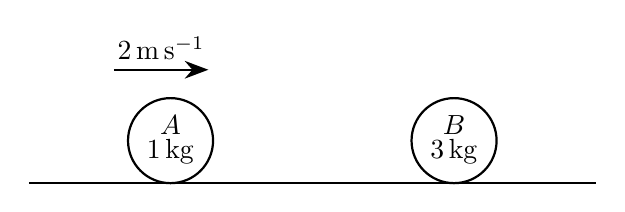
\begin{tikzpicture}[scale=1.2]
\def\rad{0.45}
\def\surf{6}
\def\arr{1.0}
\coordinate (L) at (0,0);
\coordinate (R) at (\surf,0);
\coordinate (A) at (1.5,\rad);
\coordinate (B) at (4.5,\rad);
\coordinate (Va) at ($(A)+(-0.6,0.75)$);
\draw[thick] (L) -- (R);
\draw[thick] (A) circle (\rad);
\draw[thick] (B) circle (\rad);
\draw[-{Stealth[length=3mm]}, thick] (Va) -- ++(\arr,0) node[midway, above] {$2\,\mathrm{m}\,\mathrm{s}^{-1}$};
\node at ($(A)+(0,0.16)$) {$A$};
\node at ($(A)+(0,-0.12)$) {$1\,\mathrm{kg}$};
\node at ($(B)+(0,0.16)$) {$B$};
\node at ($(B)+(0,-0.12)$) {$3\,\mathrm{kg}$};
\end{tikzpicture}
\end{figure}


The first diagram shows two spheres, $A$ and $B$, of equal radii on a smooth horizontal surface. Their masses are $1\,\mathrm{kg}$ and $3\,\mathrm{kg}$ respectively. \\

Take motion from left to right in each diagram to be positive. \\

Initially, sphere $A$ travels at speed $2\,\mathrm{m}\,\mathrm{s}^{-1}$ towards $B$, which is at rest. The spheres collide and the coefficient of restitution between $A$ and $B$ is $e$. \\
\begin{enumerate}[label=\textbf{(\alph*)}]
  \item Show that, after the collision, the velocity of $A$ is $\dfrac{1}{2}(1-3e)\,\mathrm{m}\,\mathrm{s}^{-1}$, and find an expression for the velocity of $B$ in terms of $e$. \marks{4} \\
  \item During the collision, the kinetic energy of the system decreases by $48\%$. Determine the value of $e$. \marks{3} \\
  \item Explain why the assumption that $A$ and $B$ have equal radii was needed in part (a). \marks{1} \\
\end{enumerate}


\begin{figure}[H]
    \centering
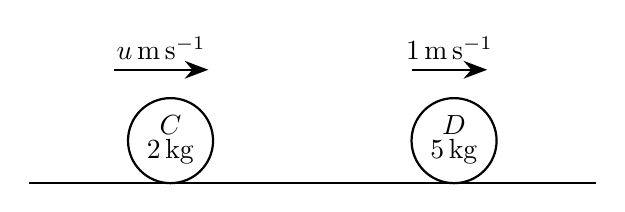
\begin{tikzpicture}[scale=1.2]
\def\rad{0.45}
\def\surf{6}
\def\arrc{1.0}
\def\arrd{0.8}
\coordinate (L) at (0,0);
\coordinate (R) at (\surf,0);
\coordinate (C) at (1.5,\rad);
\coordinate (D) at (4.5,\rad);
\coordinate (Vc) at ($(C)+(-0.6,0.75)$);
\coordinate (Vd) at ($(D)+(-0.45,0.75)$);
\draw[thick] (L) -- (R);
\draw[thick] (C) circle (\rad);
\draw[thick] (D) circle (\rad);
\draw[-{Stealth[length=3mm]}, thick] (Vc) -- ++(\arrc,0) node[midway, above] {$u\,\mathrm{m}\,\mathrm{s}^{-1}$};
\draw[-{Stealth[length=3mm]}, thick] (Vd) -- ++(\arrd,0) node[midway, above] {$1\,\mathrm{m}\,\mathrm{s}^{-1}$};
\node at ($(C)+(0,0.16)$) {$C$};
\node at ($(C)+(0,-0.12)$) {$2\,\mathrm{kg}$};
\node at ($(D)+(0,0.16)$) {$D$};
\node at ($(D)+(0,-0.12)$) {$5\,\mathrm{kg}$};
\end{tikzpicture}
\end{figure}


The second diagram shows two spheres, $C$ and $D$, of equal radii on a smooth horizontal surface. Their masses are $2\,\mathrm{kg}$ and $5\,\mathrm{kg}$ respectively. \\

Sphere $C$ is behind $D$ and both move along the same straight line in the same direction, with $C$ having speed $u\,\mathrm{m}\,\mathrm{s}^{-1}$ and $D$ having speed $1\,\mathrm{m}\,\mathrm{s}^{-1}$, where $u>1$.  \\

The spheres collide and during the collision $C$ exerts an impulse on $D$ of magnitude $\dfrac{10}{7}(u-1)\,\mathrm{N}\,\mathrm{s}$. \\
\begin{enumerate}[label=\textbf{(\alph*)}, resume]
  \item Show that $C$ and $D$ have the same velocity after the collision. \marks{4} \\
  \item Determine the fraction of kinetic energy lost due to the collision between $C$ and $D$ as $u \to \infty$. \marks{3} \\
\end{enumerate}

\vspace*{10pt}

\begin{tcolorbox}[colback=white, colframe=scarlet, title={\textbf{Solution}}, breakable, grow to left by=6mm, grow to right by=10mm]
\begin{enumerate}[label=\textbf{(\alph*)}]
  \item Let the velocities of $A$ and $B$ after the collision be $v_A$ and $v_B$ respectively, taking motion to the right as positive.

  Conservation of momentum gives
  \[
  1(2)+3(0)=1v_A+3v_B
  \]
  so
  \[
  2=v_A+3v_B
  \]

  Using the coefficient of restitution,
  \[
  \text{speed of separation}=e\times \text{speed of approach}
  \]
  Hence
  \[
  v_B-v_A=e(2-0)=2e
  \]

  So
  \[
  v_B=v_A+2e
  \]

  Substituting into the momentum equation,
  \begin{align*}
  2&=v_A+3(v_A+2e)\\
  2&=4v_A+6e\\
  4v_A&=2-6e\\
  v_A&=\frac{1-3e}{2}
  \end{align*}

  This shows that the velocity of $A$ after the collision is
  \[
  \frac{1}{2}(1-3e)\,\mathrm{m}\,\mathrm{s}^{-1}
  \]

  Then
  \begin{align*}
  v_B&=v_A+2e\\
  &=\frac{1-3e}{2}+2e\\
  &=\frac{1+e}{2}
  \end{align*}

  So the velocity of $B$ is
  \[
  \frac{1+e}{2}\,\mathrm{m}\,\mathrm{s}^{-1}
  \]

  \item Initially only $A$ is moving, so the initial kinetic energy is
  \[
  \frac12(1)(2^2)=2\text{ J}
  \]

  Since the kinetic energy decreases by $48\%$, the final kinetic energy is $52\%$ of the initial value:
  \[
  \text{final KE}=0.52\times 2=\frac{26}{25}\text{ J}
  \]

  From part (a),
  \[
  v_A=\frac{1-3e}{2},\qquad v_B=\frac{1+e}{2}
  \]

  So
  \begin{align*}
  \text{final KE}
  &=\frac12\left(\frac{1-3e}{2}\right)^2+\frac12(3)\left(\frac{1+e}{2}\right)^2\\
  &=\frac18(1-3e)^2+\frac38(1+e)^2\\
  &=\frac18(1-6e+9e^2)+\frac38(1+2e+e^2)\\
  &=\frac18\bigl(1-6e+9e^2+3+6e+3e^2\bigr)\\
  &=\frac18(4+12e^2)\\
  &=\frac12+\frac32e^2
  \end{align*}

  Therefore
  \[
  \frac12+\frac32e^2=\frac{26}{25}
  \]

  Solving,
  \begin{align*}
  \frac32e^2&=\frac{26}{25}-\frac12=\frac{27}{50}\\
  e^2&=\frac{27}{50}\times \frac23=\frac{9}{25}
  \end{align*}

  Since $0\le e\le 1$,
  \[
  e=\frac35
  \]

  \item The equal radii mean that, at impact, the centres of the spheres are at the same height, so the line of centres is horizontal.

  Therefore the impulse acts along the line of motion, so the collision is a direct one-dimensional collision. Without equal radii, the collision could be oblique.

  \item Let the impulse exerted by $C$ on $D$ be
  \[
  J=\frac{10}{7}(u-1)
  \]

  Let the velocities after collision be $v_C$ and $v_D$.

  For sphere $D$, the impulse is to the right, so
  \[
  J=\text{change in momentum of }D=5v_D-5(1)
  \]
  Hence
  \begin{align*}
  5v_D-5&=\frac{10}{7}(u-1)\\
  5v_D&=5+\frac{10}{7}(u-1)\\
  v_D&=1+\frac{2}{7}(u-1)\\
  &=\frac{2u+5}{7}
  \end{align*}

  For sphere $C$, the impulse on it is equal and opposite, so
  \[
  2v_C-2u=-J
  \]
  Hence
  \begin{align*}
  2u-2v_C&=\frac{10}{7}(u-1)\\
  2v_C&=2u-\frac{10}{7}(u-1)\\
  v_C&=u-\frac{5}{7}(u-1)\\
  &=\frac{2u+5}{7}
  \end{align*}

  Therefore
  \[
  v_C=v_D=\frac{2u+5}{7}
  \]

  So $C$ and $D$ have the same velocity after the collision.

  \item From part (d), the common velocity after the collision is
  \[
  v=\frac{2u+5}{7}
  \]

  The initial kinetic energy is
  \[
  \frac12(2)u^2+\frac12(5)(1^2)=u^2+\frac52
  \]

  The final kinetic energy is
  \begin{align*}
  \frac12(2+5)v^2
  &=\frac72\left(\frac{2u+5}{7}\right)^2\\
  &=\frac{(2u+5)^2}{14}
  \end{align*}

  So the kinetic energy lost is
  \begin{align*}
  u^2+\frac52-\frac{(2u+5)^2}{14}
  &=\frac{14u^2+35-(4u^2+20u+25)}{14}\\
  &=\frac{10u^2-20u+10}{14}\\
  &=\frac{10(u-1)^2}{14}\\
  &=\frac{5(u-1)^2}{7}
  \end{align*}

  Therefore the fraction of kinetic energy lost is
  \begin{align*}
  \frac{\frac{5(u-1)^2}{7}}{u^2+\frac52}
  &=\frac{10(u-1)^2}{7(2u^2+5)}
  \end{align*}

  Now let $u\to\infty$:
  \[
  \frac{10(u-1)^2}{7(2u^2+5)}
  =\frac{10\left(1-\frac1u\right)^2}{7\left(2+\frac{5}{u^2}\right)}
  \to \frac{10}{14}=\frac57
  \]

  Hence the fraction of kinetic energy lost tends to
  \[
  \frac57
  \]
\end{enumerate}
\end{tcolorbox}


\newpage

% ---- Question 3 ----
\questionitem

Two trolleys, $A$ and $B$, are modelled as particles of masses $0.5\,\mathrm{kg}$ and $1.0\,\mathrm{kg}$ respectively, moving along the same straight horizontal track. \\

Trolley $A$ is travelling at $7\,\mathrm{m}\,\mathrm{s}^{-1}$ and catches up with trolley $B$, which is travelling in the same direction at $2\,\mathrm{m}\,\mathrm{s}^{-1}$. The trolleys collide directly. \\

After the collision, trolley $B$ moves at $5\,\mathrm{m}\,\mathrm{s}^{-1}$ in the original direction of motion. \\

The coefficient of restitution between the trolleys is $e$. \\
\begin{enumerate}[label=\textbf{(\alph*)}]
  \item Assuming that the track is smooth, show that $e=0.8$. \marks{5} \\
  \item Describe one way in which the model could be refined. \marks{1} \\
\end{enumerate}

\vspace*{10pt}

\begin{tcolorbox}[colback=white, colframe=scarlet, title={\textbf{Solution}}, breakable, grow to left by=6mm, grow to right by=10mm]
\begin{enumerate}[label=\textbf{(\alph*)}]
  \item Take the original direction of motion as positive, and let the velocity of trolley $A$ after the collision be $v_A\,\mathrm{m}\,\mathrm{s}^{-1}$.

  Since the track is smooth, there is no external horizontal force during the collision, so linear momentum is conserved.

  \begin{align*}
  \text{Total momentum before collision} &= \text{Total momentum after collision} \\
  0.5(7) + 1.0(2) &= 0.5v_A + 1.0(5)
  \end{align*}

  So
  \begin{align*}
  3.5 + 2 &= 0.5v_A + 5 \\
  5.5 &= 0.5v_A + 5 \\
  0.5 &= 0.5v_A \\
  v_A &= 1
  \end{align*}

  The coefficient of restitution is
  \[
  e=\frac{\text{speed of separation}}{\text{speed of approach}}
  \]

  Before the collision, the speed of approach is
  \[
  7-2=5
  \]

  After the collision, the speed of separation is
  \[
  5-1=4
  \]

  Hence
  \[
  e=\frac{4}{5}=0.8
  \]

  Therefore, $e=0.8$.

  \item One refinement would be to include friction or other resistive forces, rather than assuming the track is perfectly smooth.
\end{enumerate}
\end{tcolorbox}


\newpage

% ---- Question 4 ----
\questionitem

A particle $P$ of mass $6\,\mathrm{kg}$ is projected vertically upwards from the ground with initial speed $15.8\,\mathrm{m\,s}^{-1}$ \\

At the same instant a particle $Q$ of mass $3\,\mathrm{kg}$ is projected vertically downwards with speed $4.2\,\mathrm{m\,s}^{-1}$ from a point $20\,\mathrm{m}$ above the ground. \\

During the subsequent motion $P$ and $Q$ collide. The coefficient of restitution between $P$ and $Q$ is $0.5$ \\

Determine the time between this collision and $P$ subsequently hitting the ground. \marks{10}

\vspace*{10pt}

\begin{tcolorbox}[colback=white, colframe=scarlet, title={\textbf{Solution}}, breakable, grow to left by=6mm, grow to right by=10mm]
Take upward as positive, and take \(t\) seconds after projection.

Both particles move with constant acceleration
\[
a=-9.8\ \mathrm{m\,s^{-2}}
\]

For \(P\), starting from the ground with initial velocity \(15.8\),
\[
y_P = 15.8t+\tfrac12(-9.8)t^2=15.8t-4.9t^2
\]

For \(Q\), starting \(20\) m above the ground with initial velocity \(-4.2\),
\[
y_Q = 20-4.2t+\tfrac12(-9.8)t^2=20-4.2t-4.9t^2
\]

At the collision, \(y_P=y_Q\), so
\begin{align*}
15.8t-4.9t^2 &= 20-4.2t-4.9t^2 \\
15.8t &= 20-4.2t \\
20t &= 20 \\
t&=1
\end{align*}

So they collide after \(1\) s.

The height of collision is
\[
y=15.8(1)-4.9(1)^2=10.9\ \mathrm{m}
\]

Now find the velocities just before impact.

For \(P\),
\[
u_P = 15.8-9.8(1)=6\ \mathrm{m\,s^{-1}}
\]

For \(Q\),
\[
u_Q = -4.2-9.8(1)=-14\ \mathrm{m\,s^{-1}}
\]

Let the velocities of \(P\) and \(Q\) just after collision be \(v_P\) and \(v_Q\) respectively.

Conservation of momentum gives
\begin{align*}
6(6)+3(-14)&=6v_P+3v_Q \\
36-42&=6v_P+3v_Q \\
-6&=6v_P+3v_Q \\
-2&=2v_P+v_Q
\end{align*}

Using the coefficient of restitution,
\[
e=\frac{\text{speed of separation}}{\text{speed of approach}}=\frac12
\]

Before impact, speed of approach is
\[
6-(-14)=20
\]

So speed of separation is
\[
\frac12 \times 20=10
\]

Hence
\[
v_Q-v_P=10
\]

So we solve
\begin{align*}
2v_P+v_Q&=-2 \\
v_Q-v_P&=10
\end{align*}

From the second equation,
\[
v_Q=v_P+10
\]

Substitute into the first:
\begin{align*}
2v_P+(v_P+10)&=-2 \\
3v_P+10&=-2 \\
3v_P&=-12 \\
v_P&=-4
\end{align*}

Then
\[
v_Q= -4+10=6
\]

So after the collision, particle \(P\) is \(10.9\) m above the ground and moving downward at \(4\ \mathrm{m\,s^{-1}}\).

Let the time from the collision until \(P\) hits the ground be \(\tau\) s.

For \(P\) after the collision,
\[
y = 10.9-4\tau-4.9\tau^2
\]

When it hits the ground, \(y=0\), so
\begin{align*}
10.9-4\tau-4.9\tau^2&=0 \\
4.9\tau^2+4\tau-10.9&=0
\end{align*}

Multiplying by \(10\),
\[
49\tau^2+40\tau-109=0
\]

Using the quadratic formula,
\begin{align*}
\tau &= \frac{-40\pm\sqrt{40^2-4(49)(-109)}}{2(49)} \\
&= \frac{-40\pm\sqrt{1600+21364}}{98} \\
&= \frac{-40\pm\sqrt{22964}}{98} \\
&= \frac{-40\pm 2\sqrt{5741}}{98} \\
&= \frac{-20\pm \sqrt{5741}}{49}
\end{align*}

Taking the positive root,
\[
\tau=\frac{\sqrt{5741}-20}{49}\approx 1.14
\]

Therefore, the time between the collision and \(P\) hitting the ground is
\[
\boxed{1.14\ \mathrm{s}}
\]
\end{tcolorbox}


\newpage

% ---- Question 5 ----
\questionitem

Two trolleys $P$ and $Q$, of masses $2m$ and $5m$ respectively, move along the same straight line on a smooth horizontal track. Trolley $P$ is behind trolley $Q$, and both are moving in the same direction. Trolley $P$ catches up with trolley $Q$ and they collide directly. \\

Immediately before the collision, the speed of $P$ is $ku$ and the speed of $Q$ is $u$. \\
Immediately after the collision, trolley $Q$ continues to move in the same direction with speed $v$ and the speed of $P$ is $v$. \\

The magnitude of the impulse received by $Q$ in the collision is $10mu$. \\
\begin{enumerate}[label=\textbf{(\alph*)}]
  \item Find $v$ in terms of $u$ only. \marks{3} \\
  \item Find the two possible values of $k$. \marks{5} \\
\end{enumerate}

\vspace*{10pt}

\begin{tcolorbox}[colback=white, colframe=scarlet, title={\textbf{Solution}}, breakable, grow to left by=6mm, grow to right by=10mm]
\begin{enumerate}[label=\textbf{(\alph*)}]
  \item Take the positive direction to be the original direction of motion.

  The impulse received by $Q$ is its change in momentum, so
  \[
  10mu=\left|5m(v-u)\right|
  \]
  Hence
  \[
  |v-u|=2u
  \]
  So
  \[
  v-u=2u \quad \text{or} \quad v-u=-2u
  \]
  giving
  \[
  v=3u \quad \text{or} \quad v=-u
  \]

  Since trolley $Q$ continues to move in the same direction after the collision, $v>0$. Therefore
  \[
  v=3u
  \]

  So the answer is $v=3u$.

  \item We now use conservation of momentum.

  Before the collision, total momentum is
  \[
  2m(ku)+5m(u)=2mku+5mu
  \]

  From part (a), the speed $v=3u$.

  For trolley $P$, its speed after collision is $v$, but its direction is not stated, so there are two cases.

  \textit{Case 1: $P$ continues in the same direction}

  Then after the collision,
  \[
  \text{momentum of }P=2m(3u), \qquad \text{momentum of }Q=5m(3u)
  \]
  so total momentum after the collision is
  \[
  2m(3u)+5m(3u)=7m(3u)=21mu
  \]

  Equating momenta:
  \[
  2mku+5mu=21mu
  \]
  Divide by $mu$:
  \[
  2k+5=21
  \]
  \[
  2k=16
  \]
  \[
  k=8
  \]

  \textit{Case 2: $P$ rebounds}

  Then after the collision, $Q$ still has momentum $5m(3u)$, but $P$ has momentum
  \[
  -2m(3u)
  \]
  So total momentum after the collision is
  \[
  5m(3u)-2m(3u)=3(5m-2m)u=9mu
  \]

  Equating momenta:
  \[
  2mku+5mu=9mu
  \]
  Divide by $mu$:
  \[
  2k+5=9
  \]
  \[
  2k=4
  \]
  \[
  k=2
  \]

  Therefore the two possible values of $k$ are
  \[
  k=2 \quad \text{or} \quad k=8
  \]
\end{enumerate}
\end{tcolorbox}


\newpage

% ---- Question 6 ----
\questionitem

\begin{figure}[H]
    \centering
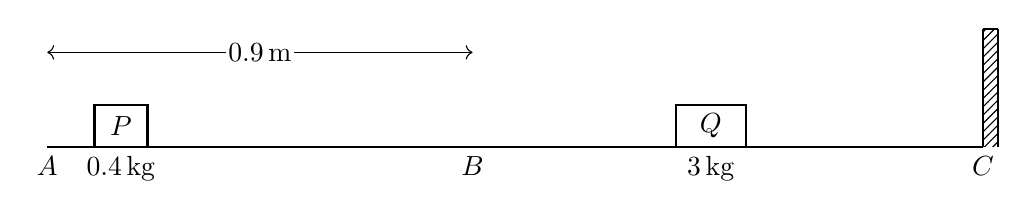
\begin{tikzpicture}[scale=1.2]
\def\AB{4}
\def\BC{5.4}
\def\bwP{0.56}
\def\bwQ{0.74}
\def\bh{0.44}
\def\wallh{1.25}
\def\wallw{0.16}

\coordinate (A) at (-0.5,0);
\coordinate (B) at (\AB,0);
\coordinate (C) at (\AB+\BC,0);

\coordinate (Psw) at ($(A)+(0.5,0)$);
\coordinate (Pne) at ($(Psw)+(\bwP,\bh)$);
\coordinate (Pbr) at ($(Psw)+(\bwP,0)$);

\coordinate (Qsw) at ($(B)+(2.15,0)$);
\coordinate (Qne) at ($(Qsw)+(\bwQ,\bh)$);
\coordinate (Qbr) at ($(Qsw)+(\bwQ,0)$);

\draw[thick] (A) -- (B);
\draw[thick] (B) -- (C);

\draw[<->] ($(A)+(0,1)$) -- node[fill=white, inner sep=1pt] {$0.9\,\mathrm{m}$} ($(B)+(0,1)$);

\draw[thick] (Psw) rectangle (Pne);
\draw[thick] (Qsw) rectangle (Qne);

\node at ($(Psw)!0.5!(Pne)$) {$P$};
\node at ($(Qsw)!0.5!(Qne)$) {$Q$};

\node[below] at ($(Psw)!0.5!(Pbr)$) {$0.4\,\mathrm{kg}$};
\node[below] at ($(Qsw)!0.5!(Qbr)$) {$3\,\mathrm{kg}$};

\fill[pattern=north east lines] (C) rectangle ++(\wallw,\wallh);
\draw[thick] (C) -- ++(0,\wallh);
\draw[thick] ($(C)+(\wallw,0)$) -- ++(0,\wallh);
\draw[thick] ($(C)+(0,\wallh)$) -- ++(\wallw,0);

\node[below] at (A) {$A$};
\node[below] at (B) {$B$};
\node[below] at (C) {$C$};
\end{tikzpicture}
\end{figure}


The diagram shows two blocks $P$ and $Q$ of masses $0.4\,\mathrm{kg}$ and $3\,\mathrm{kg}$ respectively, on a horizontal surface. The points $A$, $B$ and $C$ lie on the surface in a straight line. The surface between $A$ and $B$ is rough and the surface between $B$ and $C$ is smooth. There is a wall at $C$. \\

The coefficient of friction between $P$ and $AB$ is $\dfrac{25}{49}$ \\

Initially, $P$ is at $A$ and $Q$ is at rest on $BC$. Block $P$ is projected directly towards $Q$ with speed $5\,\mathrm{m}\,\mathrm{s}^{-1}$. The two blocks collide on $BC$. As a result of the collision, $P$ changes direction and comes to rest at $A$. You may assume that $P$ only collides with $Q$ once. \\
\begin{enumerate}[label=\textbf{(\alph*)}]
  \item Determine the coefficient of restitution between $P$ and $Q$. \marks{6} \\
  \item Calculate the impulse exerted on $P$ by $Q$ during the collision. \marks{2} \\
\end{enumerate}
After the collision with $P$, block $Q$ strikes the wall at $C$. The collision between $Q$ and the wall is perfectly elastic. After rebounding from the wall, $Q$ comes to rest at a point on $AB$ that is $0.30\,\mathrm{m}$ from $A$. \\
\begin{enumerate}[label=\textbf{(\alph*)}, resume]
  \item Determine the coefficient of friction between $Q$ and $AB$. \marks{3} \\
\end{enumerate}

\vspace*{10pt}

\begin{tcolorbox}[colback=white, colframe=scarlet, title={\textbf{Solution}}, breakable, grow to left by=6mm, grow to right by=10mm]
\begin{enumerate}[label=\textbf{(\alph*)}]
  \item Take motion to the right as positive.

  For block $P$ on $AB$, the frictional deceleration is
  \[
  a=\mu g=\frac{25}{49}\times 9.8=5\ \mathrm{m\,s^{-2}}
  \]

  From $A$ to $B$, $P$ travels $0.9\,\mathrm{m}$ on the rough surface, so
  \[
  v^2=u^2+2as
  \]
  gives
  \[
  v^2=5^2+2(-5)(0.9)=25-9=16
  \]
  Hence
  \[
  v=4\ \mathrm{m\,s^{-1}}
  \]
  Since $BC$ is smooth, the speed of $P$ just before the collision is still
  \[
  u_P=4\ \mathrm{m\,s^{-1}}
  \]
  Also $Q$ is initially at rest, so
  \[
  u_Q=0
  \]

  After the collision, $P$ changes direction and eventually comes to rest at $A$.
  Since $BC$ is smooth, the speed of $P$ immediately after the collision is the same as its speed when it reaches $B$ on the way back.

  Let this speed be $u$. On $AB$, it then comes to rest after $0.9\,\mathrm{m}$, so
  \[
  0=u^2+2(-5)(0.9)
  \]
  \[
  0=u^2-9
  \]
  \[
  u^2=9
  \]
  \[
  u=3
  \]
  Since $P$ is moving to the left after the collision,
  \[
  v_P=-3\ \mathrm{m\,s^{-1}}
  \]

  Let the velocity of $Q$ immediately after the collision be $v_Q$.

  Using conservation of momentum:
  \[
  0.4(4)+3(0)=0.4(-3)+3v_Q
  \]
  \[
  1.6=-1.2+3v_Q
  \]
  \[
  2.8=3v_Q
  \]
  \[
  v_Q=\frac{14}{15}\ \mathrm{m\,s^{-1}}
  \]

  Now use
  \[
  e=\frac{\text{speed of separation}}{\text{speed of approach}}
  \]
  so
  \[
  e=\frac{v_Q-v_P}{u_P-u_Q}
  =\frac{\frac{14}{15}-(-3)}{4-0}
  \]
  \[
  e=\frac{\frac{14}{15}+3}{4}
  =\frac{\frac{59}{15}}{4}
  =\frac{59}{60}
  \]

  Therefore, the coefficient of restitution is
  \[
  \frac{59}{60}
  \]

  \item The impulse exerted on $P$ by $Q$ is the change in momentum of $P$:
  \[
  I=0.4(-3)-0.4(4)
  \]
  \[
  I=0.4(-7)=-2.8\ \mathrm{N\,s}
  \]

  The negative sign shows the impulse is to the left.

  Therefore, the impulse is
  \[
  2.8\ \mathrm{N\,s}\ \text{to the left}
  \]

  \item From part (a), $Q$ leaves the collision with speed
  \[
  \frac{14}{15}\ \mathrm{m\,s^{-1}}
  \]
  towards the wall.

  The collision with the wall is perfectly elastic, so $Q$ rebounds with the same speed:
  \[
  \frac{14}{15}\ \mathrm{m\,s^{-1}}
  \]
  Since $BC$ is smooth, its speed at $B$ on the way back is still
  \[
  \frac{14}{15}\ \mathrm{m\,s^{-1}}
  \]

  It comes to rest at a point on $AB$ which is $0.30\,\mathrm{m}$ from $A$, so the distance travelled on the rough part is
  \[
  0.9-0.30=0.60\ \mathrm{m}
  \]

  Let the coefficient of friction between $Q$ and $AB$ be $\mu$.
  Then the deceleration on $AB$ is $\mu g$.

  Using
  \[
  v^2=u^2+2as
  \]
  with $v=0$, $u=\dfrac{14}{15}$, $a=-\mu g$ and $s=0.60$:
  \[
  0=\left(\frac{14}{15}\right)^2+2(-\mu g)(0.60)
  \]
  \[
  0=\left(\frac{14}{15}\right)^2-2\mu\left(\frac{49}{5}\right)\left(\frac{3}{5}\right)
  \]
  \[
  \frac{196}{225}=\frac{294}{25}\mu
  \]
  \[
  \mu=\frac{196}{225}\times\frac{25}{294}
  =\frac{2}{27}
  \]

  Therefore, the coefficient of friction is
  \[
  \frac{2}{27}\approx 0.0741
  \]
\end{enumerate}
\end{tcolorbox}


\newpage

% ---- Question 7 ----
\questionitem

Particle $P$ has mass $m$ and particle $Q$ has mass $7m$. \\

The particles are moving in the same direction along the same straight line on a smooth horizontal surface. \\
Particle $P$ collides directly with particle $Q$. \\
Immediately before the collision, the speed of $P$ is $9u$ and the speed of $Q$ is $u$. \\
After the collision, the direction of motion of $P$ is reversed. \\

The coefficient of restitution between $P$ and $Q$ is $e$. \\
\begin{enumerate}[label=\textbf{(\alph*)}]
  \item Find the complete range of possible values of $e$. \marks{7} \\
  \item Given that $e=\dfrac{3}{4}$, find the total kinetic energy lost in the collision between $P$ and $Q$. \marks{4} \\
\end{enumerate}
After the collision, $P$ hits a smooth fixed vertical wall that is perpendicular to the direction of motion of $P$. Particle $P$ rebounds. \\
The coefficient of restitution between $P$ and the wall is $f$. \\

Given that there is a second collision between $P$ and $Q$, \\
\begin{enumerate}[label=\textbf{(\alph*)}, resume]
  \item find the complete range of possible values of $f$. \marks{3} \\
\end{enumerate}

\vspace*{10pt}

\begin{tcolorbox}[colback=white, colframe=scarlet, title={\textbf{Solution}}, breakable, grow to left by=6mm, grow to right by=10mm]
\begin{enumerate}[label=\textbf{(\alph*)}]
  \item Take the original direction of motion as positive, and let the velocities of $P$ and $Q$ immediately after the first collision be $v_P$ and $v_Q$ respectively.

  Conservation of momentum gives
  \begin{align*}
  m(9u)+7m(u)&=mv_P+7mv_Q \\
  16mu&=m(v_P+7v_Q)
  \end{align*}
  so
  \[
  16u=v_P+7v_Q
  \]

  Using the definition of coefficient of restitution,
  \[
  e=\frac{\text{speed of separation}}{\text{speed of approach}}
  \]

  Before collision, the speed of approach is
  \[
  9u-u=8u
  \]

  After collision, the speed of separation is
  \[
  v_Q-v_P
  \]

  Hence
  \[
  v_Q-v_P=8eu
  \]

  So we have the simultaneous equations
  \begin{align*}
  v_P+7v_Q&=16u \\
  -v_P+v_Q&=8eu
  \end{align*}

  From the second equation,
  \[
  v_Q=v_P+8eu
  \]

  Substitute into the first equation:
  \begin{align*}
  v_P+7(v_P+8eu)&=16u \\
  8v_P+56eu&=16u \\
  8v_P&=16u-56eu \\
  v_P&=(2-7e)u
  \end{align*}

  Then
  \begin{align*}
  v_Q&=v_P+8eu \\
  &=(2-7e)u+8eu \\
  &=(2+e)u
  \end{align*}

  We are told that after the collision the direction of motion of $P$ is reversed, so $v_P<0$.
  Therefore
  \begin{align*}
  (2-7e)u&<0
  \end{align*}
  and since $u>0$,
  \begin{align*}
  2-7e&<0 \\
  e&>\frac{2}{7}
  \end{align*}

  Also, for a coefficient of restitution,
  \[
  0\leq e\leq 1
  \]

  Combining these gives
  \[
  \frac{2}{7}<e\leq 1
  \]

  So the complete range of possible values is $\displaystyle \frac{2}{7}<e\leq 1$.

  \item Given $e=\dfrac34$, from part (a),
  \begin{align*}
  v_P&=(2-7e)u=\left(2-\frac{21}{4}\right)u=-\frac{13u}{4} \\
  v_Q&=(2+e)u=\left(2+\frac34\right)u=\frac{11u}{4}
  \end{align*}

  The initial kinetic energy is
  \begin{align*}
  \frac12 m(9u)^2+\frac12(7m)(u)^2
  &=\frac12 m(81u^2)+\frac72 mu^2 \\
  &=\frac{81}{2}mu^2+\frac{7}{2}mu^2 \\
  &=44mu^2
  \end{align*}

  The final kinetic energy is
  \begin{align*}
  \frac12 m\left(\frac{13u}{4}\right)^2+\frac12(7m)\left(\frac{11u}{4}\right)^2
  &=\frac12 m\cdot \frac{169u^2}{16}+\frac{7}{2}m\cdot \frac{121u^2}{16} \\
  &=\frac{169}{32}mu^2+\frac{847}{32}mu^2 \\
  &=\frac{1016}{32}mu^2 \\
  &=\frac{127}{4}mu^2
  \end{align*}

  So the kinetic energy lost is
  \begin{align*}
  44mu^2-\frac{127}{4}mu^2
  &=\frac{176}{4}mu^2-\frac{127}{4}mu^2 \\
  &=\frac{49}{4}mu^2
  \end{align*}

  Therefore the total kinetic energy lost is $\displaystyle \frac{49}{4}mu^2$.

  \item After the first collision, $P$ has velocity
  \[
  -\frac{13u}{4}
  \]

  So $P$ hits the wall moving towards it with speed $\dfrac{13u}{4}$.

  For the collision with the fixed wall, the coefficient of restitution is $f$, so
  \[
  f=\frac{\text{speed of rebound}}{\text{speed of approach}}
  \]

  Hence after rebounding, the speed of $P$ is
  \[
  f\cdot \frac{13u}{4}=\frac{13fu}{4}
  \]

  and its direction is reversed, so $P$ now moves in the positive direction with velocity
  \[
  \frac{13fu}{4}
  \]

  Particle $Q$ is still moving in the positive direction with velocity
  \[
  \frac{11u}{4}
  \]

  For there to be a second collision, $P$ must catch up with $Q$, so $P$ must be moving faster than $Q$:
  \begin{align*}
  \frac{13fu}{4}&>\frac{11u}{4}
  \end{align*}

  Since $u>0$,
  \begin{align*}
  13f&>11 \\
  f&>\frac{11}{13}
  \end{align*}

  Also $0\leq f\leq 1$ for a coefficient of restitution.

  Therefore the complete range of possible values is
  \[
  \frac{11}{13}<f\leq 1
  \]
\end{enumerate}
\end{tcolorbox}


\newpage

% ---- Question 8 ----
\questionitem

A particle $A$ of mass $3m$ is moving with speed $4u$ on a smooth horizontal plane towards a smooth fixed vertical wall. A particle $B$ of mass $m$ is on the same line between $A$ and the wall, moving directly towards $A$ with speed $u$. \\

Particles $A$ and $B$ collide directly. The coefficient of restitution between $A$ and $B$ is $e$, where $0<e\le 1$. \\
\begin{enumerate}[label=\textbf{(\alph*)}]
  \item Show that immediately after the collision $B$ moves towards the wall with speed $\dfrac{u}{4}(11+15e)$. \marks{6} \\
  \item Show that there will be a second collision between $A$ and $B$ after $B$ has collided with the wall. \marks{3} \\
\end{enumerate}
The coefficient of restitution between $B$ and the wall is
\(
\dfrac{1}{3}
\) \\

Find, in simplified form, in terms of $m$, $u$ and $e$, \\
\begin{enumerate}[label=\textbf{(\alph*)}, resume]
  \item the magnitude of the impulse received by $B$ from the wall, \marks{3} \\
  \item the loss in kinetic energy of $B$ due to its collision with the wall. \marks{3} \\
\end{enumerate}

\vspace*{10pt}

\begin{tcolorbox}[colback=white, colframe=scarlet, title={\textbf{Solution}}, breakable, grow to left by=6mm, grow to right by=10mm]
\begin{enumerate}[label=\textbf{(\alph*)}]
  \item Take motion \emph{towards the wall} as positive.

  Before the collision,
  \[
  u_A=4u,\qquad u_B=-u
  \]

  Let the velocities immediately after the collision be $v_A$ and $v_B$.

  Conserving linear momentum:
  \begin{align*}
  3m(4u)+m(-u)&=3mv_A+mv_B\\
  12mu-mu&=3mv_A+mv_B\\
  11u&=3v_A+v_B
  \end{align*}

  Using the coefficient of restitution,
  \[
  \text{speed of separation}=e\times \text{speed of approach}
  \]
  so
  \begin{align*}
  v_B-v_A&=e\bigl(4u-(-u)\bigr)\\
  v_B-v_A&=5eu
  \end{align*}

  Hence
  \[
  v_B=v_A+5eu
  \]

  Substitute into the momentum equation:
  \begin{align*}
  3v_A+(v_A+5eu)&=11u\\
  4v_A&=11u-5eu\\
  v_A&=\frac{u}{4}(11-5e)
  \end{align*}

  Then
  \begin{align*}
  v_B&=v_A+5eu\\
  &=\frac{u}{4}(11-5e)+5eu\\
  &=\frac{u}{4}(11-5e+20e)\\
  &=\frac{u}{4}(11+15e)
  \end{align*}

  Since $0<e\le 1$, this is positive, so $B$ moves towards the wall.

  Therefore, immediately after the collision, $B$ moves towards the wall with speed
  \[
  \frac{u}{4}(11+15e)
  \]

  \item From part (a),
  \[
  v_A=\frac{u}{4}(11-5e),\qquad v_B=\frac{u}{4}(11+15e)
  \]

  Also
  \[
  v_B-v_A=5eu>0
  \]
  so $B$ is moving faster than $A$, and therefore $B$ reaches the wall first.

  Let the distance from the point of the first collision to the wall be $d$.

  When $B$ reaches the wall, $A$ has travelled
  \[
  d\cdot \frac{v_A}{v_B}
  \]
  which is less than $d$ because $v_A<v_B$.

  So at that instant $A$ has \emph{not} yet reached the wall.

  Now $B$ collides with the wall and rebounds. Since the coefficient of restitution with the wall is $\frac13$, its speed after rebounding is
  \[
  \frac{v_B}{3}
  \]
  in the opposite direction.

  So after the wall collision, $A$ is still moving towards the wall with speed $v_A$, while $B$ is moving away from the wall towards $A$ with speed $\frac{v_B}{3}$.

  The distance between them at that moment is
  \begin{align*}
  d-d\frac{v_A}{v_B}
  &=d\left(1-\frac{v_A}{v_B}\right)
  \end{align*}

  Their relative speed is
  \[
  v_A+\frac{v_B}{3}
  \]

  Hence the time until they meet is
  \begin{align*}
  \frac{d\left(1-\frac{v_A}{v_B}\right)}{v_A+\frac{v_B}{3}}
  \end{align*}

  Substitute for $v_A$ and $v_B$:
  \begin{align*}
  1-\frac{v_A}{v_B}
  &=\frac{v_B-v_A}{v_B}
  =\frac{5eu}{(11+15e)u/4}
  =\frac{20e}{11+15e}
  \end{align*}
  and
  \begin{align*}
  v_A+\frac{v_B}{3}
  &=\frac{u}{4}(11-5e)+\frac{1}{3}\cdot \frac{u}{4}(11+15e)\\
  &=\frac{u}{12}\bigl(3(11-5e)+(11+15e)\bigr)\\
  &=\frac{44u}{12}\\
  &=\frac{11u}{3}
  \end{align*}

  Therefore
  \begin{align*}
  \text{time to second collision}
  &=\frac{d\left(\frac{20e}{11+15e}\right)}{11u/3}\\
  &=\frac{60de}{11u(11+15e)}
  \end{align*}

  Since $d>0$, $u>0$ and $e>0$, this time is positive.

  Therefore there \emph{will} be a second collision between $A$ and $B$ after $B$ has collided with the wall.

  \item Let
  \[
  V=\frac{u}{4}(11+15e)
  \]
  be the speed of $B$ just before it hits the wall.

  Taking motion towards the wall as positive, the velocity of $B$ changes from
  \[
  +V \quad \text{to} \quad -\frac{V}{3}
  \]

  So the change in velocity is
  \begin{align*}
  -\frac{V}{3}-V
  =-\frac{4V}{3}
  \end{align*}

  Hence the magnitude of the impulse is
  \begin{align*}
  m\left|\Delta v\right|
  &=m\left(\frac{4V}{3}\right)\\
  &=\frac{4m}{3}\cdot \frac{u}{4}(11+15e)\\
  &=\frac{mu}{3}(11+15e)
  \end{align*}

  Therefore the magnitude of the impulse received by $B$ from the wall is
  \[
  \frac{mu}{3}(11+15e)
  \]

  \item Using $V=\dfrac{u}{4}(11+15e)$, the kinetic energy of $B$ before hitting the wall is
  \[
  \frac12 mV^2
  \]
  and after rebounding it is
  \[
  \frac12 m\left(\frac{V}{3}\right)^2
  \]

  So the loss in kinetic energy is
  \begin{align*}
  \frac12 mV^2-\frac12 m\left(\frac{V}{3}\right)^2
  &=\frac12 mV^2\left(1-\frac19\right)\\
  &=\frac12 mV^2\cdot \frac89\\
  &=\frac49 mV^2
  \end{align*}

  Now
  \[
  V^2=\left(\frac{u}{4}(11+15e)\right)^2=\frac{u^2(11+15e)^2}{16}
  \]

  Therefore
  \begin{align*}
  \text{loss in kinetic energy}
  &=\frac49 m\cdot \frac{u^2(11+15e)^2}{16}\\
  &=\frac{mu^2(11+15e)^2}{36}
  \end{align*}

  Therefore the loss in kinetic energy of $B$ is
  \[
  \frac{mu^2(11+15e)^2}{36}
  \]
\end{enumerate}
\end{tcolorbox}


\newpage

% ---- Question 9 ----
\questionitem

A particle $P$ of mass $m$ is moving in a straight line with speed $5u$ on a smooth horizontal plane. It collides directly with a particle $Q$ of mass $4m$ that is initially at rest on the plane. \\

The coefficient of restitution between $P$ and $Q$ is $e$, where $e>\dfrac{2}{3}$. \\

\begin{enumerate}[label=\textbf{(\alph*)}]
  \item Show that the speed of $P$ immediately after the collision is
  \[
  (4e-1)u
  \]
  \marks[-20pt]{4}
\end{enumerate}
After the collision, $P$ moves in the opposite direction and strikes a smooth fixed vertical wall that is perpendicular to the direction of motion of $P$. The coefficient of restitution between $P$ and the wall is $f$. \\

\begin{enumerate}[label=\textbf{(\alph*)}, resume]
  \item Find, in terms of $e$, the set of values of $f$ for which there will be a second collision between $P$ and $Q$. \marks{6} \\
\end{enumerate}

\vspace*{10pt}

\begin{tcolorbox}[colback=white, colframe=scarlet, title={\textbf{Solution}}, breakable, grow to left by=6mm, grow to right by=10mm]
\begin{enumerate}[label=\textbf{(\alph*)}]
  \item Take the positive direction to be the original direction of motion of $P$.

Let the velocities of $P$ and $Q$ immediately after the first collision be $v_P$ and $v_Q$ respectively.

By conservation of momentum,
\[
m(5u)+4m(0)=mv_P+4mv_Q
\]
so
\[
5u=v_P+4v_Q
\]

Using the definition of coefficient of restitution,
\[
e=\frac{\text{speed of separation}}{\text{speed of approach}}
=\frac{v_Q-v_P}{5u}
\]
hence
\[
v_Q-v_P=5eu
\]

Now solve the two equations.

From
\[
v_Q=v_P+5eu
\]
substitute into the momentum equation:
\[
5u=v_P+4(v_P+5eu)
\]
\[
5u=5v_P+20eu
\]
\[
5v_P=5u-20eu
\]
\[
v_P=(1-4e)u
\]

Also,
\[
v_Q=v_P+5eu=(1-4e)u+5eu=(1+e)u
\]

Since $e>\frac23$, we have
\[
1-4e<0
\]
so $v_P$ is negative. This means $P$ moves in the opposite direction after the collision.

Therefore the \emph{speed} of $P$ is
\[
-(1-4e)u=(4e-1)u
\]

So the speed of $P$ immediately after the collision is $(4e-1)u$.

  \item After the first collision:

\begin{itemize}
\item $P$ moves to the left with speed $(4e-1)u$
\item $Q$ moves to the right with speed $(1+e)u$
\end{itemize}

When $P$ strikes the fixed wall, the coefficient of restitution with the wall is $f$, so

\[
f=\frac{\text{speed of rebound}}{\text{speed of approach}}
\]

Hence, after rebounding from the wall, $P$ moves to the right with speed
\[
f(4e-1)u
\]

For there to be a second collision, $P$ must catch up with $Q$ after rebounding from the wall.

Since both then move to the right on a smooth plane, this requires
\[
f(4e-1)u>(1+e)u
\]

As $u>0$, divide through by $u$:
\[
f(4e-1)>1+e
\]

Also $e>\frac23$, so $4e-1>0$, and we can divide by $4e-1$:
\[
f>\frac{1+e}{4e-1}
\]

Now $f$ is a coefficient of restitution, so
\[
f\le 1
\]

We should check that the lower bound is less than $1$:
\[
\frac{1+e}{4e-1}<1
\iff 1+e<4e-1
\iff 2<3e
\iff e>\frac23
\]
which is true.

Therefore the required set of values of $f$ is
\[
\frac{1+e}{4e-1}<f\le 1
\]

So,
\[
\frac{1+e}{4e-1}<f\le 1
\]
\end{enumerate}
\end{tcolorbox}


\newpage

% ---- Question 10 ----
\questionitem

\begin{figure}[H]
    \centering
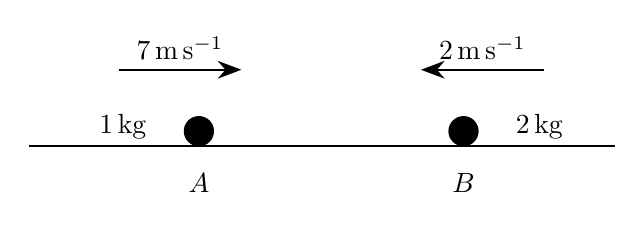
\begin{tikzpicture}[scale=1.2]
\def\rad{0.16}
\coordinate (A) at (1.2,\rad);
\coordinate (B) at (4.0,\rad);
\draw[thick] (-0.6,0) -- (5.6,0);
\fill (A) circle (\rad);
\fill (B) circle (\rad);
\draw[-{Stealth[length=3mm]}, thick] ($(A)+(-0.85,0.65)$) -- ++(1.3,0) node[midway, above] {$7\,\mathrm{m\,s^{-1}}$};
\draw[-{Stealth[length=3mm]}, thick] ($(B)+(0.85,0.65)$) -- ++(-1.3,0) node[midway, above] {$2\,\mathrm{m\,s^{-1}}$};
\node[left] at ($(A)+(-0.45,0.05)$) {$1\,\mathrm{kg}$};
\node[right] at ($(B)+(0.45,0.05)$) {$2\,\mathrm{kg}$};
\node[below] at ($(A)+(0,-0.35)$) {$A$};
\node[below] at ($(B)+(0,-0.35)$) {$B$};
\end{tikzpicture}
\end{figure}


Two small uniform smooth spheres $A$ and $B$ have masses $1\,\mathrm{kg}$ and $2\,\mathrm{kg}$ respectively. The spheres are moving towards each other in the same straight line on a smooth horizontal surface. Sphere $A$ is moving to the right with speed $7\,\mathrm{m\,s^{-1}}$ and sphere $B$ is moving to the left with speed $2\,\mathrm{m\,s^{-1}}$. The spheres collide. After the collision, $A$ moves with speed $1\,\mathrm{m\,s^{-1}}$. \\

Determine the possible speeds with which $B$ moves after the collision. \marks{4}

\vspace*{10pt}

\begin{tcolorbox}[colback=white, colframe=scarlet, title={\textbf{Solution}}, breakable, grow to left by=6mm, grow to right by=10mm]
Take motion to the right as positive.

Since the surface is smooth, there is no external horizontal impulse, so horizontal momentum is conserved.

Before the collision:
\[
\text{momentum} = (1)(7) + (2)(-2) = 7-4=3
\]

Let the velocity of $A$ after the collision be $v_A$ and the velocity of $B$ after the collision be $v_B$.

Then conservation of momentum gives
\[
1v_A+2v_B=3
\]

We are told that after the collision, $A$ has speed $1\,\mathrm{m\,s^{-1}}$, so its velocity could be either
\[
v_A=1 \quad \text{or} \quad v_A=-1
\]

\textbf{Case 1:} $v_A=1$

Substitute into the momentum equation:
\[
1+2v_B=3
\]
\[
2v_B=2
\]
\[
v_B=1
\]

So $B$ has speed $1\,\mathrm{m\,s^{-1}}$.

\textbf{Case 2:} $v_A=-1$

Substitute into the momentum equation:
\[
-1+2v_B=3
\]
\[
2v_B=4
\]
\[
v_B=2
\]

So $B$ has speed $2\,\mathrm{m\,s^{-1}}$.

Therefore, the possible speeds of $B$ after the collision are
\[
1\,\mathrm{m\,s^{-1}} \quad \text{or} \quad 2\,\mathrm{m\,s^{-1}}
\]
\end{tcolorbox}


\newpage

% ---- Question 11 ----
\questionitem

Particles $P$ and $Q$, of masses $m$ and $3m$ respectively, move on a smooth horizontal plane in the same straight line towards a vertical wall. Particle $Q$ is in front of $P$. Initially, $P$ has speed $6u$ and $Q$ has speed $u$. Particle $P$ catches up with $Q$ and the particles collide before either particle reaches the wall. \\

The coefficient of restitution between the particles is $e$. \\

As a result of the collision, the direction of motion of $P$ is reversed. \\

\begin{enumerate}[label=\textbf{(\alph*)}]
  \item Find, in terms of $u$ and $e$, the speed of $P$ after the collision. \marks{6} \\
\end{enumerate}
After the collision, $Q$ continues to the wall and rebounds. The coefficient of restitution between $Q$ and the wall is $\dfrac{1}{3}$. \\

Given that there is a second collision between $P$ and $Q$, \\

\begin{enumerate}[label=\textbf{(\alph*)}, resume]
  \item find the full range of possible values of $e$. \marks{5} \\
\end{enumerate}

\vspace*{10pt}

\begin{tcolorbox}[colback=white, colframe=scarlet, title={\textbf{Solution}}, breakable, grow to left by=6mm, grow to right by=10mm]
\begin{enumerate}[label=\textbf{(\alph*)}]
  \item Take motion towards the wall as positive.

  Let the velocities of $P$ and $Q$ after the first collision be $v_P$ and $v_Q$ respectively.

  Conservation of momentum gives
  \[
  m(6u)+3m(u)=mv_P+3mv_Q
  \]
  so
  \[
  9u=v_P+3v_Q
  \]

  Using the definition of coefficient of restitution,
  \[
  \text{speed of separation}=e\times \text{speed of approach}
  \]
  hence
  \[
  v_Q-v_P=e(6u-u)=5eu
  \]

  So we have the simultaneous equations
  \begin{align*}
  9u&=v_P+3v_Q \\
  5eu&=v_Q-v_P
  \end{align*}

  From the first equation,
  \[
  v_P=9u-3v_Q
  \]

  Substitute into the restitution equation:
  \begin{align*}
  v_Q-(9u-3v_Q)&=5eu \\
  4v_Q-9u&=5eu \\
  4v_Q&=(9+5e)u \\
  v_Q&=\frac{(9+5e)u}{4}
  \end{align*}

  Then
  \begin{align*}
  v_P&=9u-3\left(\frac{(9+5e)u}{4}\right) \\
     &=\frac{36u-(27+15e)u}{4} \\
     &=\frac{(9-15e)u}{4} \\
     &=\frac{3(3-5e)u}{4}
  \end{align*}

  We are told that the direction of motion of $P$ is reversed, so $v_P<0$. Therefore the speed of $P$ is
  \[
  -v_P=\frac{3u(5e-3)}{4}
  \]

  Hence the speed of $P$ after the collision is $\displaystyle \frac{3u(5e-3)}{4}$

  \item From part (a), for $P$ to reverse direction we need
  \[
  v_P=\frac{3(3-5e)u}{4}<0
  \]
  so
  \[
  3-5e<0
  \]
  and therefore
  \[
  e>\frac35
  \]

  Also from part (a), the speed of $Q$ after the first collision is
  \[
  \frac{(9+5e)u}{4}
  \]

  When $Q$ hits the wall, the coefficient of restitution between $Q$ and the wall is $\frac13$, so the speed of $Q$ after rebounding is
  \[
  \frac13\times \frac{(9+5e)u}{4}=\frac{(9+5e)u}{12}
  \]

  After the rebound, both particles move away from the wall. For there to be a second collision, $Q$ must catch $P$, so the rebounding speed of $Q$ must be greater than the speed of $P$.

  Hence
  \[
  \frac{(9+5e)u}{12}>\frac{3u(5e-3)}{4}
  \]

  Since $u>0$, multiply by $\frac{12}{u}$:
  \begin{align*}
  9+5e&>9(5e-3) \\
  9+5e&>45e-27 \\
  36&>40e \\
  e&<\frac{9}{10}
  \end{align*}

  Combining this with $e>\frac35$ gives
  \[
  \frac35<e<\frac9{10}
  \]

  Hence the full range of possible values of $e$ is $\displaystyle \frac35<e<\frac9{10}$
\end{enumerate}
\end{tcolorbox}


\newpage

% ---- Question 12 ----
\questionitem

Two small uniform smooth spheres $A$ and $B$, of masses $2\,\mathrm{kg}$ and $6\,\mathrm{kg}$ respectively, are on a smooth horizontal surface. Sphere $A$ is projected directly towards $B$ with speed $4\,\mathrm{m}\,\mathrm{s}^{-1}$. Sphere $B$ is initially at rest. The coefficient of restitution between $A$ and $B$ is $e$. \\
\begin{enumerate}[label=\textbf{(\alph*)}]
  \item Show that the velocity of $A$ after the collision, in the original direction of motion of $A$, is $(1-3e)\,\mathrm{m}\,\mathrm{s}^{-1}$ and find a similar expression for the velocity of $B$. \marks{5} \\
  \item The following three parts are independent of each other, and each considers a different scenario regarding the collision between $A$ and $B$. \\
  \begin{enumerate}[label=(\roman*)]
    \item In the collision between $A$ and $B$ the spheres coalesce to form a combined body $C$. State the speed of $C$ after the collision. \marks{1}
    \item In the collision between $A$ and $B$ the direction of motion of $A$ is reversed. Find the range of possible values of $e$. \marks{2}
    \item The total loss in kinetic energy due to the collision is $9\,\mathrm{J}$. Determine the value of $e$. \marks{4} \\
  \end{enumerate}
\end{enumerate}

\vspace*{10pt}

\begin{tcolorbox}[colback=white, colframe=scarlet, title={\textbf{Solution}}, breakable, grow to left by=6mm, grow to right by=10mm]
\begin{enumerate}[label=\textbf{(\alph*)}]
  \item Take the original direction of motion of $A$ as positive.

Let the velocities of $A$ and $B$ after the collision be $v_A$ and $v_B$ respectively.

Since the surface is smooth, horizontal momentum is conserved:
\begin{align*}
2(4)+6(0)&=2v_A+6v_B \\
8&=2v_A+6v_B \\
4&=v_A+3v_B
\end{align*}

Using the definition of coefficient of restitution,
\[
e=\frac{\text{speed of separation}}{\text{speed of approach}}
\]

Before collision, the speed of approach is $4-0=4$.

After collision, the speed of separation is $v_B-v_A$, so
\begin{align*}
e&=\frac{v_B-v_A}{4} \\
v_B-v_A&=4e
\end{align*}

So we solve the simultaneous equations
\begin{align*}
v_A+3v_B&=4 \\
-v_A+v_B&=4e
\end{align*}

Adding gives
\begin{align*}
4v_B&=4+4e \\
v_B&=1+e
\end{align*}

Substituting into $v_B-v_A=4e$:
\begin{align*}
(1+e)-v_A&=4e \\
1-v_A&=3e \\
v_A&=1-3e
\end{align*}

Hence the velocity of $A$ after the collision is $(1-3e)\,\mathrm{m}\,\mathrm{s}^{-1}$, and the velocity of $B$ is $(1+e)\,\mathrm{m}\,\mathrm{s}^{-1}$.

  \item \begin{enumerate}[label=\textbf{(\roman*)}]
    \item If the spheres coalesce, they move together with a common speed $v$.

By conservation of momentum,
\begin{align*}
2(4)+6(0)&=(2+6)v \\
8&=8v \\
v&=1
\end{align*}

So the speed of $C$ is $1\,\mathrm{m}\,\mathrm{s}^{-1}$.

    \item From part (a), the velocity of $A$ after collision is
\[
v_A=1-3e
\]

If the direction of motion of $A$ is reversed, then $v_A<0$, so
\begin{align*}
1-3e&<0 \\
1&<3e \\
e&>\frac13
\end{align*}

Also, for a coefficient of restitution,
\[
0\le e\le 1
\]

Hence the possible values of $e$ are
\[
\frac13<e\le 1
\]

    \item Initial kinetic energy:
\begin{align*}
\text{KE}_{\text{initial}}&=\frac12(2)(4^2) \\
&=16\ \mathrm{J}
\end{align*}

From part (a), after collision the velocities are $1-3e$ and $1+e$.

So the final kinetic energy is
\begin{align*}
\text{KE}_{\text{final}}
&=\frac12(2)(1-3e)^2+\frac12(6)(1+e)^2 \\
&=(1-3e)^2+3(1+e)^2 \\
&=(1-6e+9e^2)+3(1+2e+e^2) \\
&=1-6e+9e^2+3+6e+3e^2 \\
&=4+12e^2
\end{align*}

Hence the loss in kinetic energy is
\begin{align*}
16-(4+12e^2)&=9 \\
12-12e^2&=9 \\
12(1-e^2)&=9 \\
1-e^2&=\frac34 \\
e^2&=\frac14
\end{align*}

So
\[
e=\pm \frac12
\]

But a coefficient of restitution must satisfy $0\le e\le 1$, so
\[
e=\frac12
\]

Therefore, $e=\frac12$.
  \end{enumerate}
\end{enumerate}
\end{tcolorbox}


\end{enumerate}
\end{document}
